\section{Results}

\subsection{Modal analysis of uncoupled elements.}

The six lowest modes of vibration of bandola's top and back plate are presented in Figures \ref{TopPlateModes} and \ref{BackPlateModes}, where each mode is identified with the label $(m, n)$ that refers to the number $m$, $n$ of antinodal areas in the $x$ and $y$ directions respectively. Initials "T" for top plate and "B" for back plate that begin the mode label are used to specify the modes for each plate. Colored bar indicates the scale of contours displacement, ranging from blue, the minimum displacement, to red, the maximum displacement. These displacements are not an absolute quantity since each mode is normalized separately, however, their importance lies in the relation between the different contours (amplitudes) in the plate.\\

\begin{figure}[h]
\centering
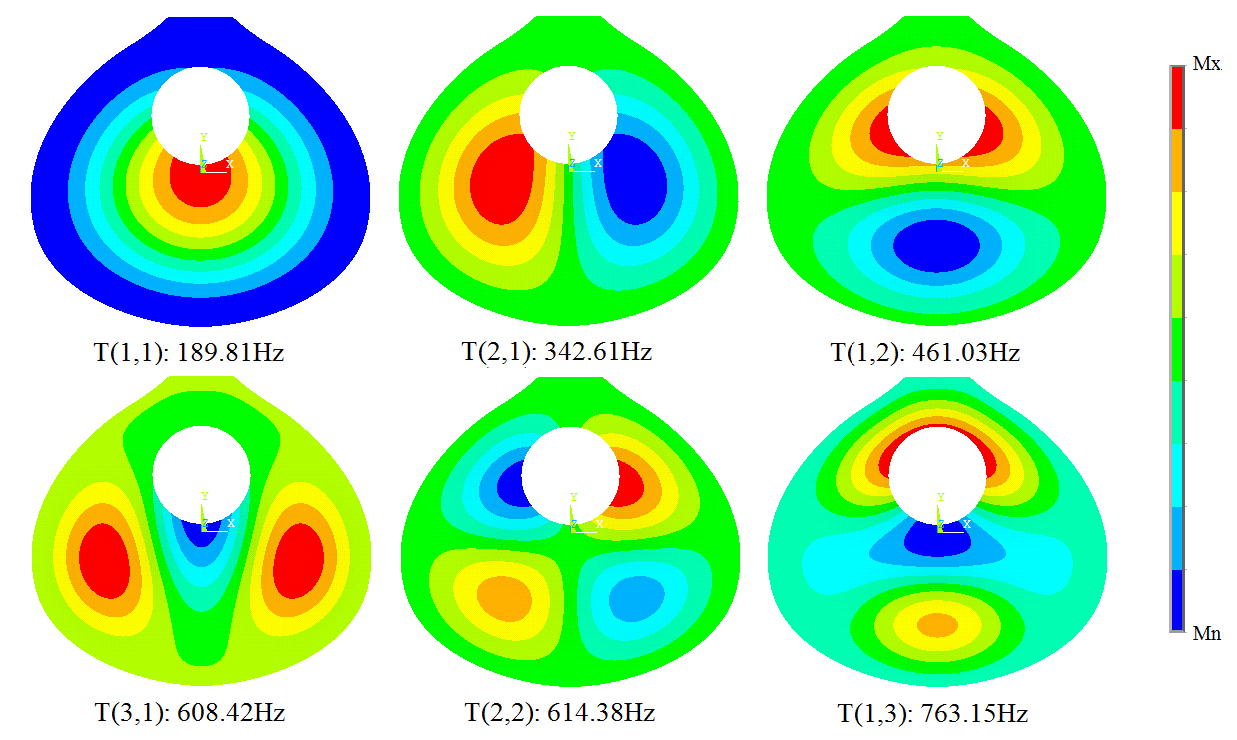
\includegraphics[height=4cm]{img/TopPlateModes.png}
\caption{Simulated modes of vibration of the top plate.}
\label{TopPlateModes}
\end{figure}

\begin{figure}[h]
\centering
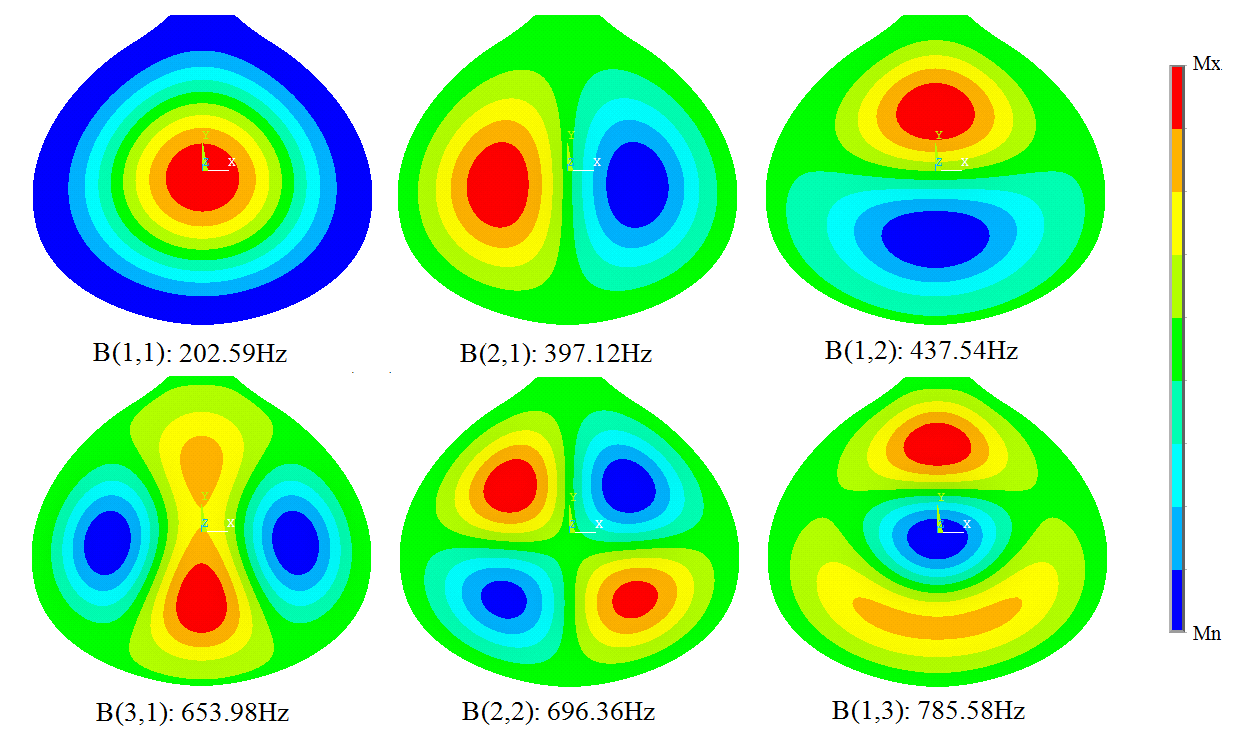
\includegraphics[height=4cm]{img/BackPlateModes.png}
\caption{Simulated modes of vibration of the back plate.}
\label{BackPlateModes}
\end{figure}

According to the material properties of each wood, frequency values for back plate modes are higher than those for top plate. Rosewood is a hardwood and hence, higher frequencies were expected. By comparing the frequencies with those for open strings in Table \ref{StringTuning}, it can be observed that calculated frequencies of the plates are within the sound register of bandola. This fact could mean that material properties used for analysis are in a good range of approximation. Despite of this, it is known that fan bracing and harmonic bars have the effect of increase resonance frequencies of the plates and thus, if numerical models had considered fan bracing, harmonic bars or any structural reinforcement, the modal frequencies would have been higher. Something similar happens in classical guitars \cite{Rossing}, where first top and back plate frequencies, usually 183Hz and 204Hz respectively, are far enough from the lowest tuning frequency of open strings, which is 82Hz.\\

Analyzing the resulted mode shapes for the bandola's plates, it can be confirmed, like in guitars, that the fundamental modes (1,1) are characterized by symmetrical variation of amplitude over the bout of the bandola. This result supports the assumption of coupling models based on \cite{Christensen, Christensen3}, where these first modes of the plates are modelled as simple harmonic oscillators that represent the displacement of the mode effective mass. Besides the fundamental modes, the others can be identified according the experimented stresses, i.e., modes (2,1) and (3,1) are recognized as "transverse flexural modes", modes (1,2) and (1,3) are the "longitudinal flexural modes", and the mode (2,2) is called the "shear mode".

Figure \ref{AirModes13} shows the obtained modes for the air in the cavity. This three lowest modes are identified as the air modes A0, A1, A2. Colored bar indicates the scale of contours pressure, ranging from blue, the minimum pressure, to red, the maximum pressure.

\begin{figure}[h]
\centering
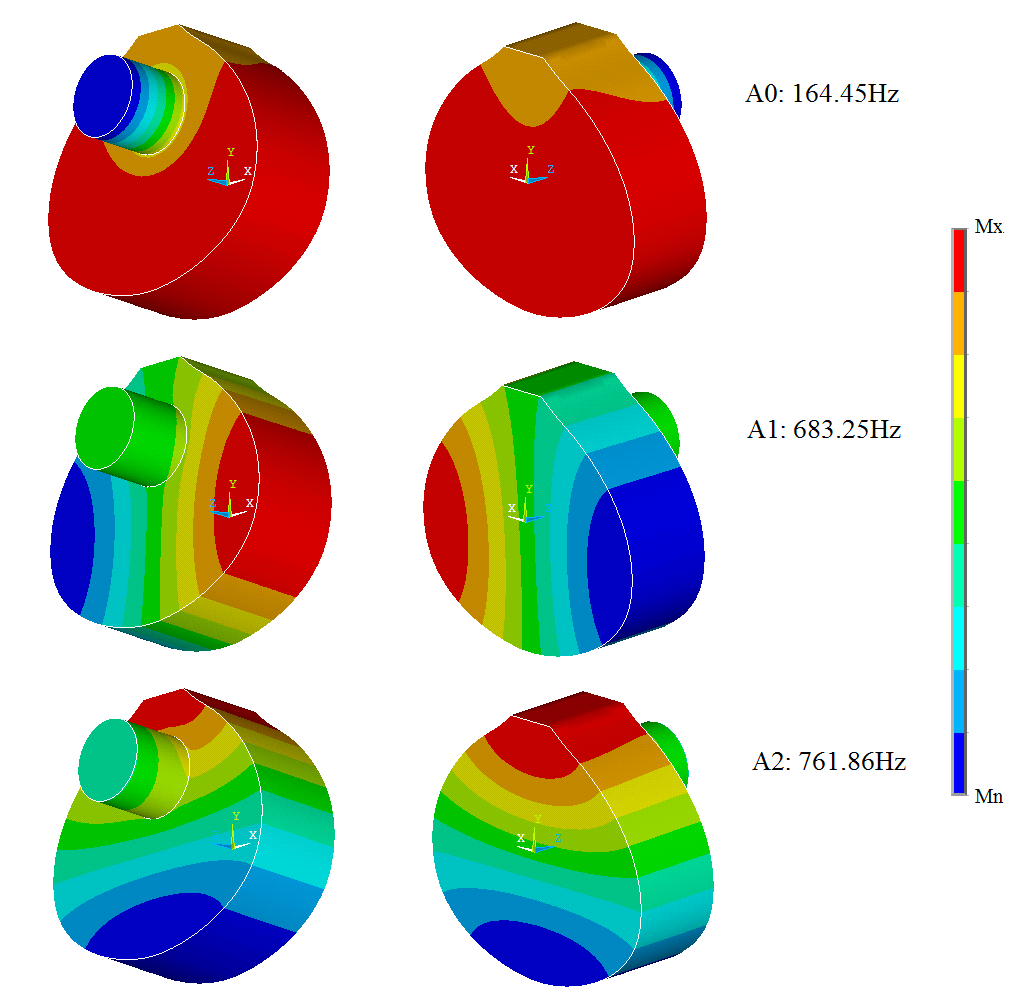
\includegraphics[height=5cm]{img/AirModes13.png}
\caption{Air modes A0, A1 and A2.}
\label{AirModes13}
\end{figure}

Air mode A0 is known as the Helmholtz resonance and according to the coupling models, it is of great importance for bandola's dynamic response at low frequencies since it couples the system. A pure Helmholtz resonator is characterized by a maximum constant pressure inside the cavity (that acts as an air cushion) and a pressure variation in the region of the neck that drives the oscillating piston of air. Considering this, the mode A0 presented in Figure \ref{AirModes13} indicates that air inside of bandola's cavity doesn't behave exactly as a Helmoholtz resonator (though it is very similar) since it presents a little variation in pressure along the cavity. This fact could be explained considering the geometry of the bandola.

It can be observed that the frequency of A0 is considerably far apart from the other modal frequencies, constituting a difference of almost two musical octaves for the nearest mode A1. This characteristic could reflect the great influence of this first mode at the lowest frequencies of the bandola by comparing both the obtained frequencies for plates and bandola's sound register in Table \ref{StringTuning}. Besides A0, A1 shows a transverse pressure distribution and A2 shows a longitudinal pressure distribution.

\subsection{Modal analysis of coupled elements.}

Figures \ref{CoupledModes2a}, \ref{CoupledModes2b} and \ref{CoupledModes2c} show the calculated modes for the system in which the top plate and the air in the cavity interact. Nine modes are presented in the range of 0-800Hz, from these modes several patterns of the uncoupled modes can be identified. The modes are labelled with the initials "TA" that indicate the coupling between Top plate and Air, the scripts "DT", "PF" and "PB" are used to specify the variable plotted, i.e., displacements in top plate, pressure in the front view and pressure in the back view, respectively. Color bar indicates the scale of contours magnitude corresponding to the plotted variable, ranging from blue, the minimum magnitude, to red, the maximum magnitude.

\begin{figure}[h]
\centering
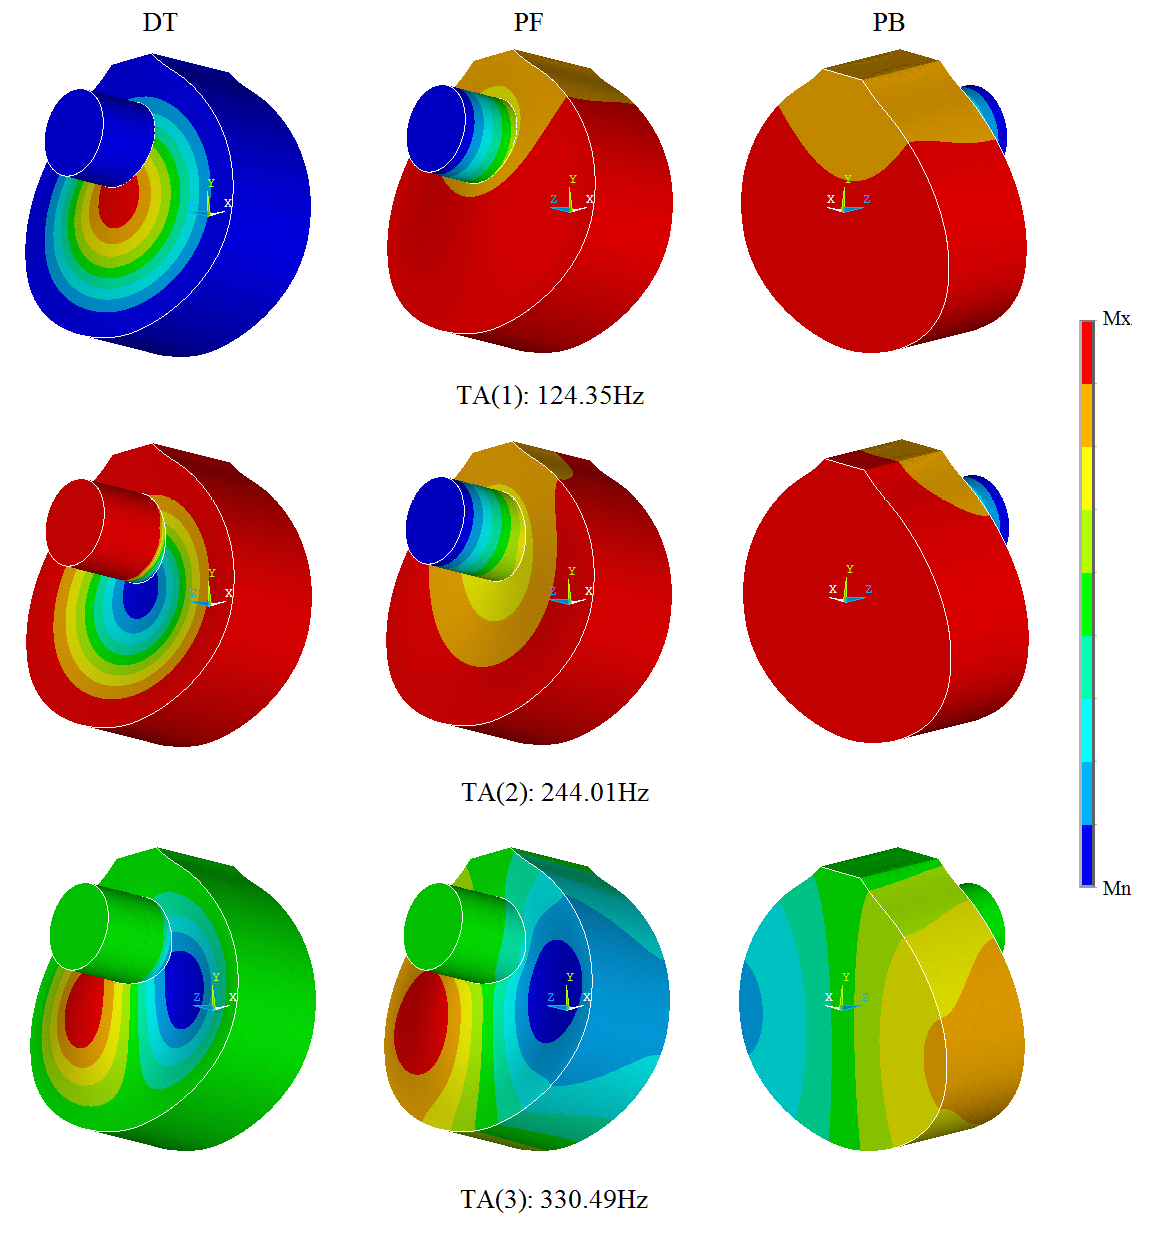
\includegraphics[height=6cm]{img/CoupledModes2a.png}
\caption{Coupled modes of vibration for bandola's resonance box considering the oscillation of top plate and enclosed air. The back plate is assumed to be rigid.}
\label{CoupledModes2a}
\end{figure}

\begin{figure}[h]
\centering
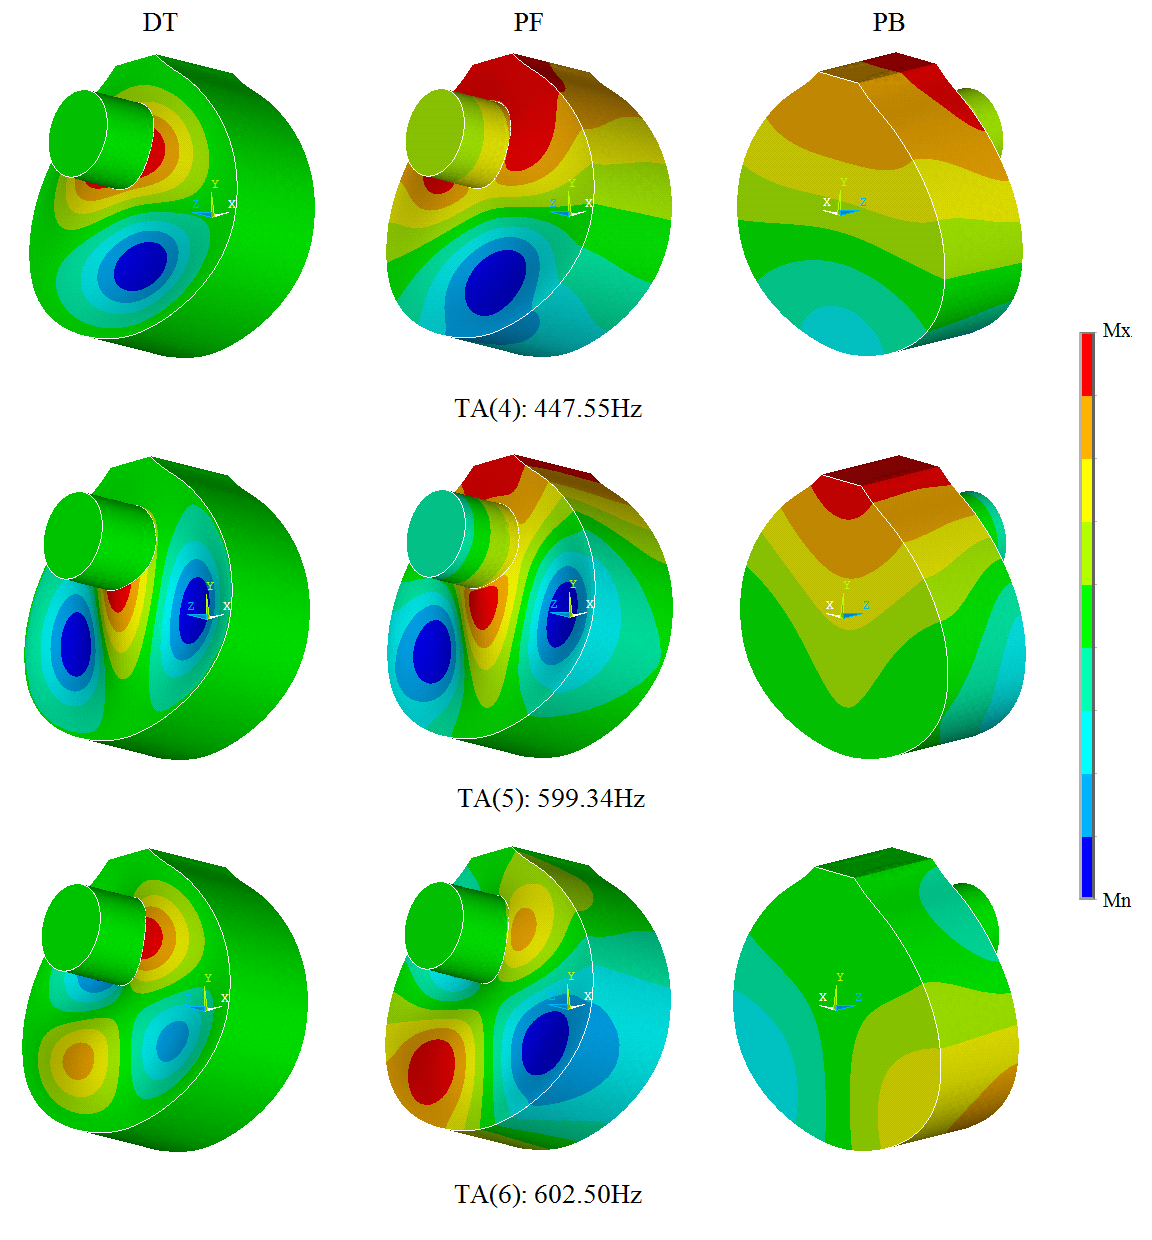
\includegraphics[height=6cm]{img/CoupledModes2b.png}
\caption{Coupled modes of vibration for bandola's resonance box considering the oscillation of top plate and enclosed air. The back plate is assumed to be rigid.}
\label{CoupledModes2b}
\end{figure}

\begin{figure}[h]
\centering
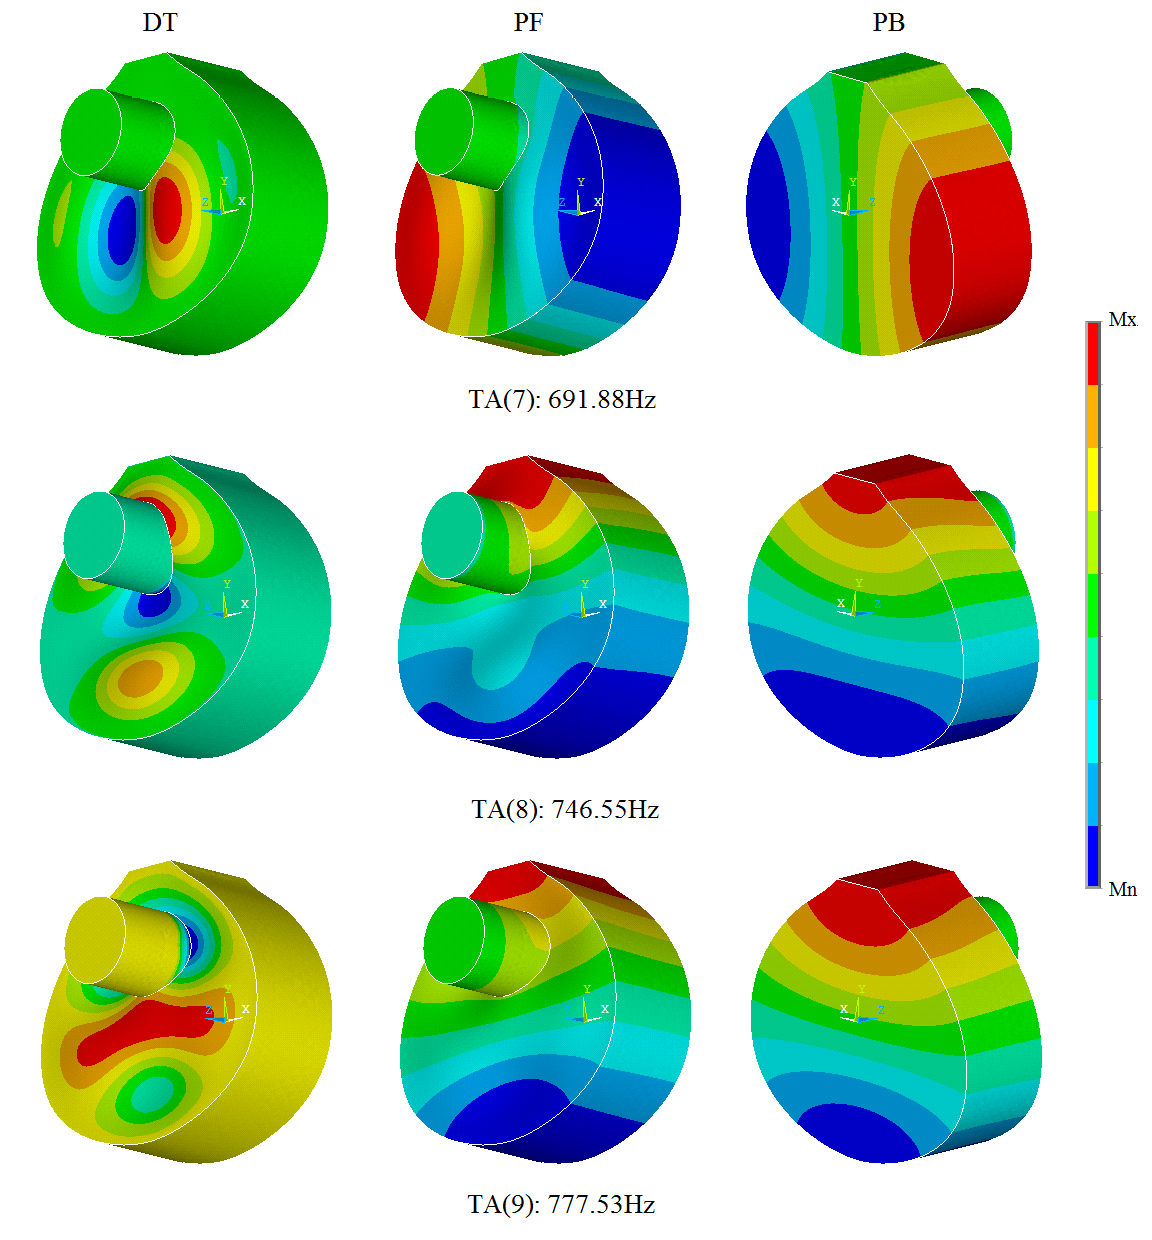
\includegraphics[height=6cm]{img/CoupledModes2c.png}
\caption{Coupled modes of vibration for bandola's resonance box considering the oscillation of top plate and enclosed air. The back plate is assumed to be rigid.}
\label{CoupledModes2c}
\end{figure}

The uncoupled modes calculated for top plate and air have shown that Helmholtz resonance of the air A0 is lower than the fundamental resonance of the top plate T(1,1). As it is exposed in the Figure \ref{CoupledModes2a}, TA(1) and TA(2) present in turn, lower and higher resonances (respectively) compared with those of uncoupled elements. With these results and according to the coupling model of two oscillators, combination of both the fundamental resonance of top plate and the Helmholtz resonance thus give rise to a lower resonance TA(1) and a higher resonance TA(2). From mode shapes, it can also be said that these two coupled modes seem to be efficient radiators since a big area of the bout of the bandola excites the air in front of it. The efficiency of this radiation will also be determined by the phase of piston air and in order to get any information of it, it would be convenient experimental measurements.

Verifying the expression in E.q.\ref{Combination2} it is found that:
\begin{eqnarray*}
\sqrt{f_p^2 + f_h^2} & = & 251.14 \text{Hz}\\
\sqrt{f_1^2 + f_2^2} & = & 273.87 \text{Hz},
\end{eqnarray*}
where the frequency $f=\omega / 2 \pi$. These results are coherent since the percent error, relative to the sum of coupled terms, is 8.3\%. At this point, it would be convenient an experimental validation.

Now, with respect to the other coupled modes in the frequency range, it can be observed throughout the following 7 modes that the combination of the remaining 5 modes of the plate with the other two of the air is presented. As it was expected, the resultant modes are combination of uncoupled modes. In this sense, models more complex could be considered in order to predict more modes, using more oscillators representing every mode in the plate or in the air. A model with nine oscillators, three representing the modes of air inside the cavity and six representing the modes of the top plate, all lying into the same frequency range, would predict the nine calculated coupled modes, also into the same range.

Some global characteristics from of all of the calculated coupled modes can be mentioned. First, the correspondence between uncoupled modes of the top plate and the air in every coupled mode, seems to respond to the longitudinal or transverse disposition of the modes, for instance, transverse top plate modes are usually related to the transverse pressure distribution of mode A1, whereas longitudinal top plates modes are related to the longitudinal pressure distribution of mode A2. The shear mode of the top plate also support this idea since it was related to a pressure distribution that can be described from the combination of both air modes A1 and A2. The other characteristic identified was that coupled modes may be usually driven by those uncoupled modes with the nearest frequency.

Figures \ref{CoupledModes3a}, \ref{CoupledModes3b} and \ref{CoupledModes3c} show the calculated modes for the system in which the top plate, the air in the cavity and the back plate interact. Fifteen modes are presented in the same range, they are labelled with the initials "TAB" that indicate the coupling between Top plate, Air and Back plate, the scripts "DT", "DB", "PF" and "PB" are used to specify the variable plotted, i.e., displacements in top plate, displacements in back plate, pressure in the front view and pressure in the back view, respectively. Colors indicate the scale of contours magnitude as in above figures.

\begin{figure}[h]
\centering
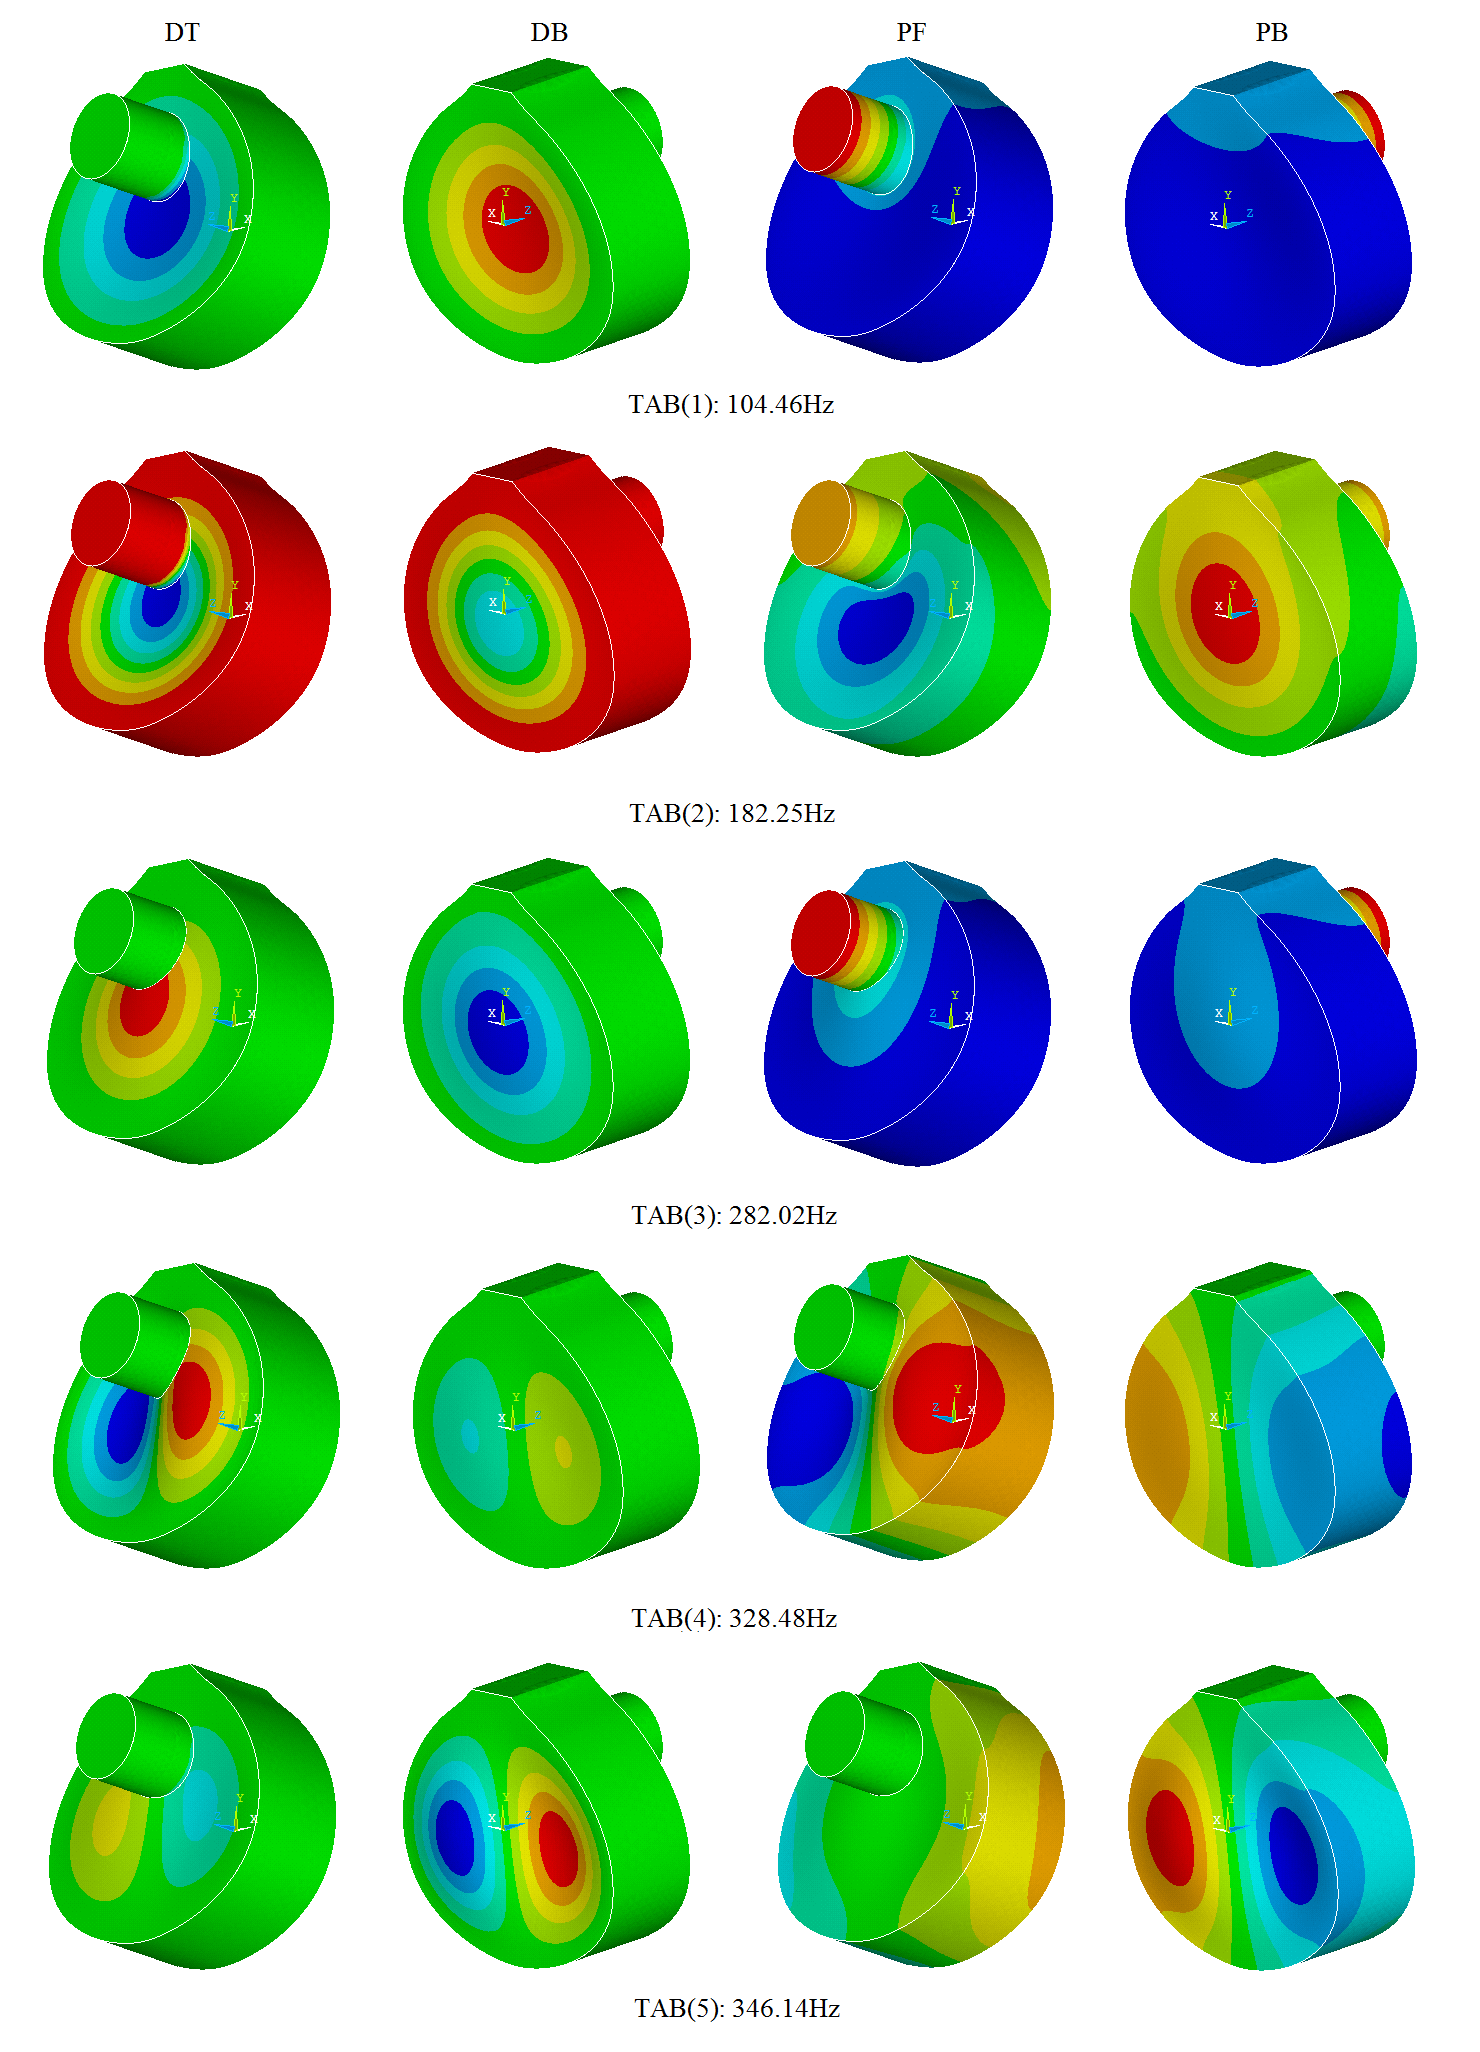
\includegraphics[height=9cm]{img/FSI3a.png}
\caption{Coupled modes of vibration for bandola's resonance box considering the oscillation of top plate, enclosed air and back plate}
\label{CoupledModes3a}
\end{figure}

\begin{figure}[h]
\centering
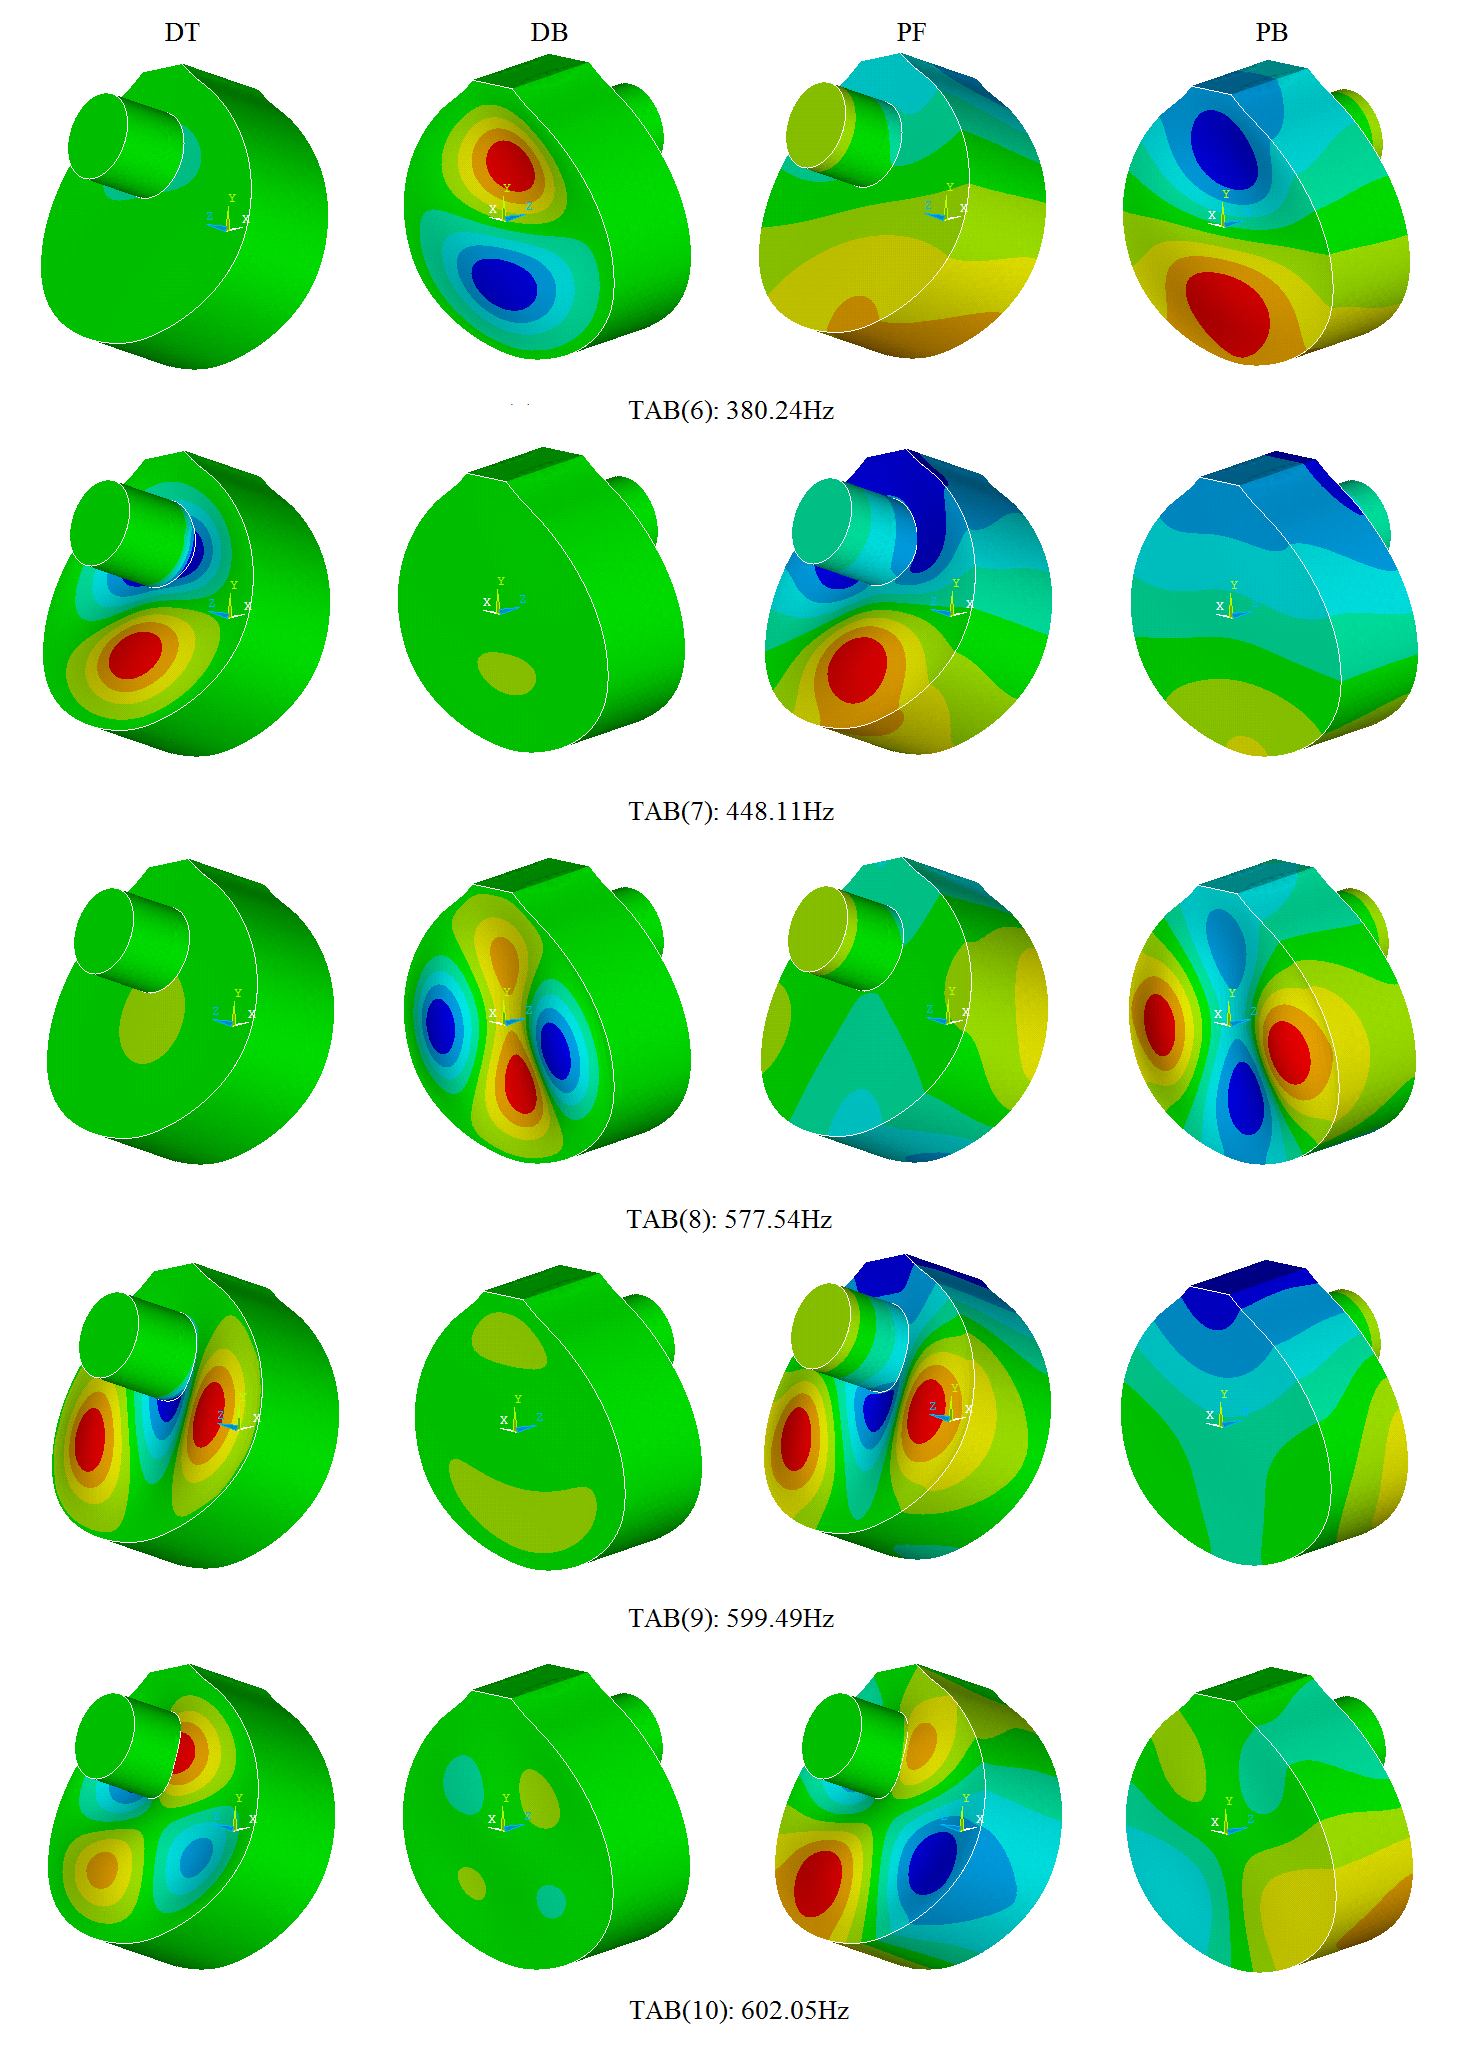
\includegraphics[height=9cm]{img/FSI3b.png}
\caption{Coupled modes of vibration for bandola's resonance box considering the oscillation of top plate, enclosed air and back plate}
\label{CoupledModes3b}
\end{figure}

\begin{figure}[h]
\centering
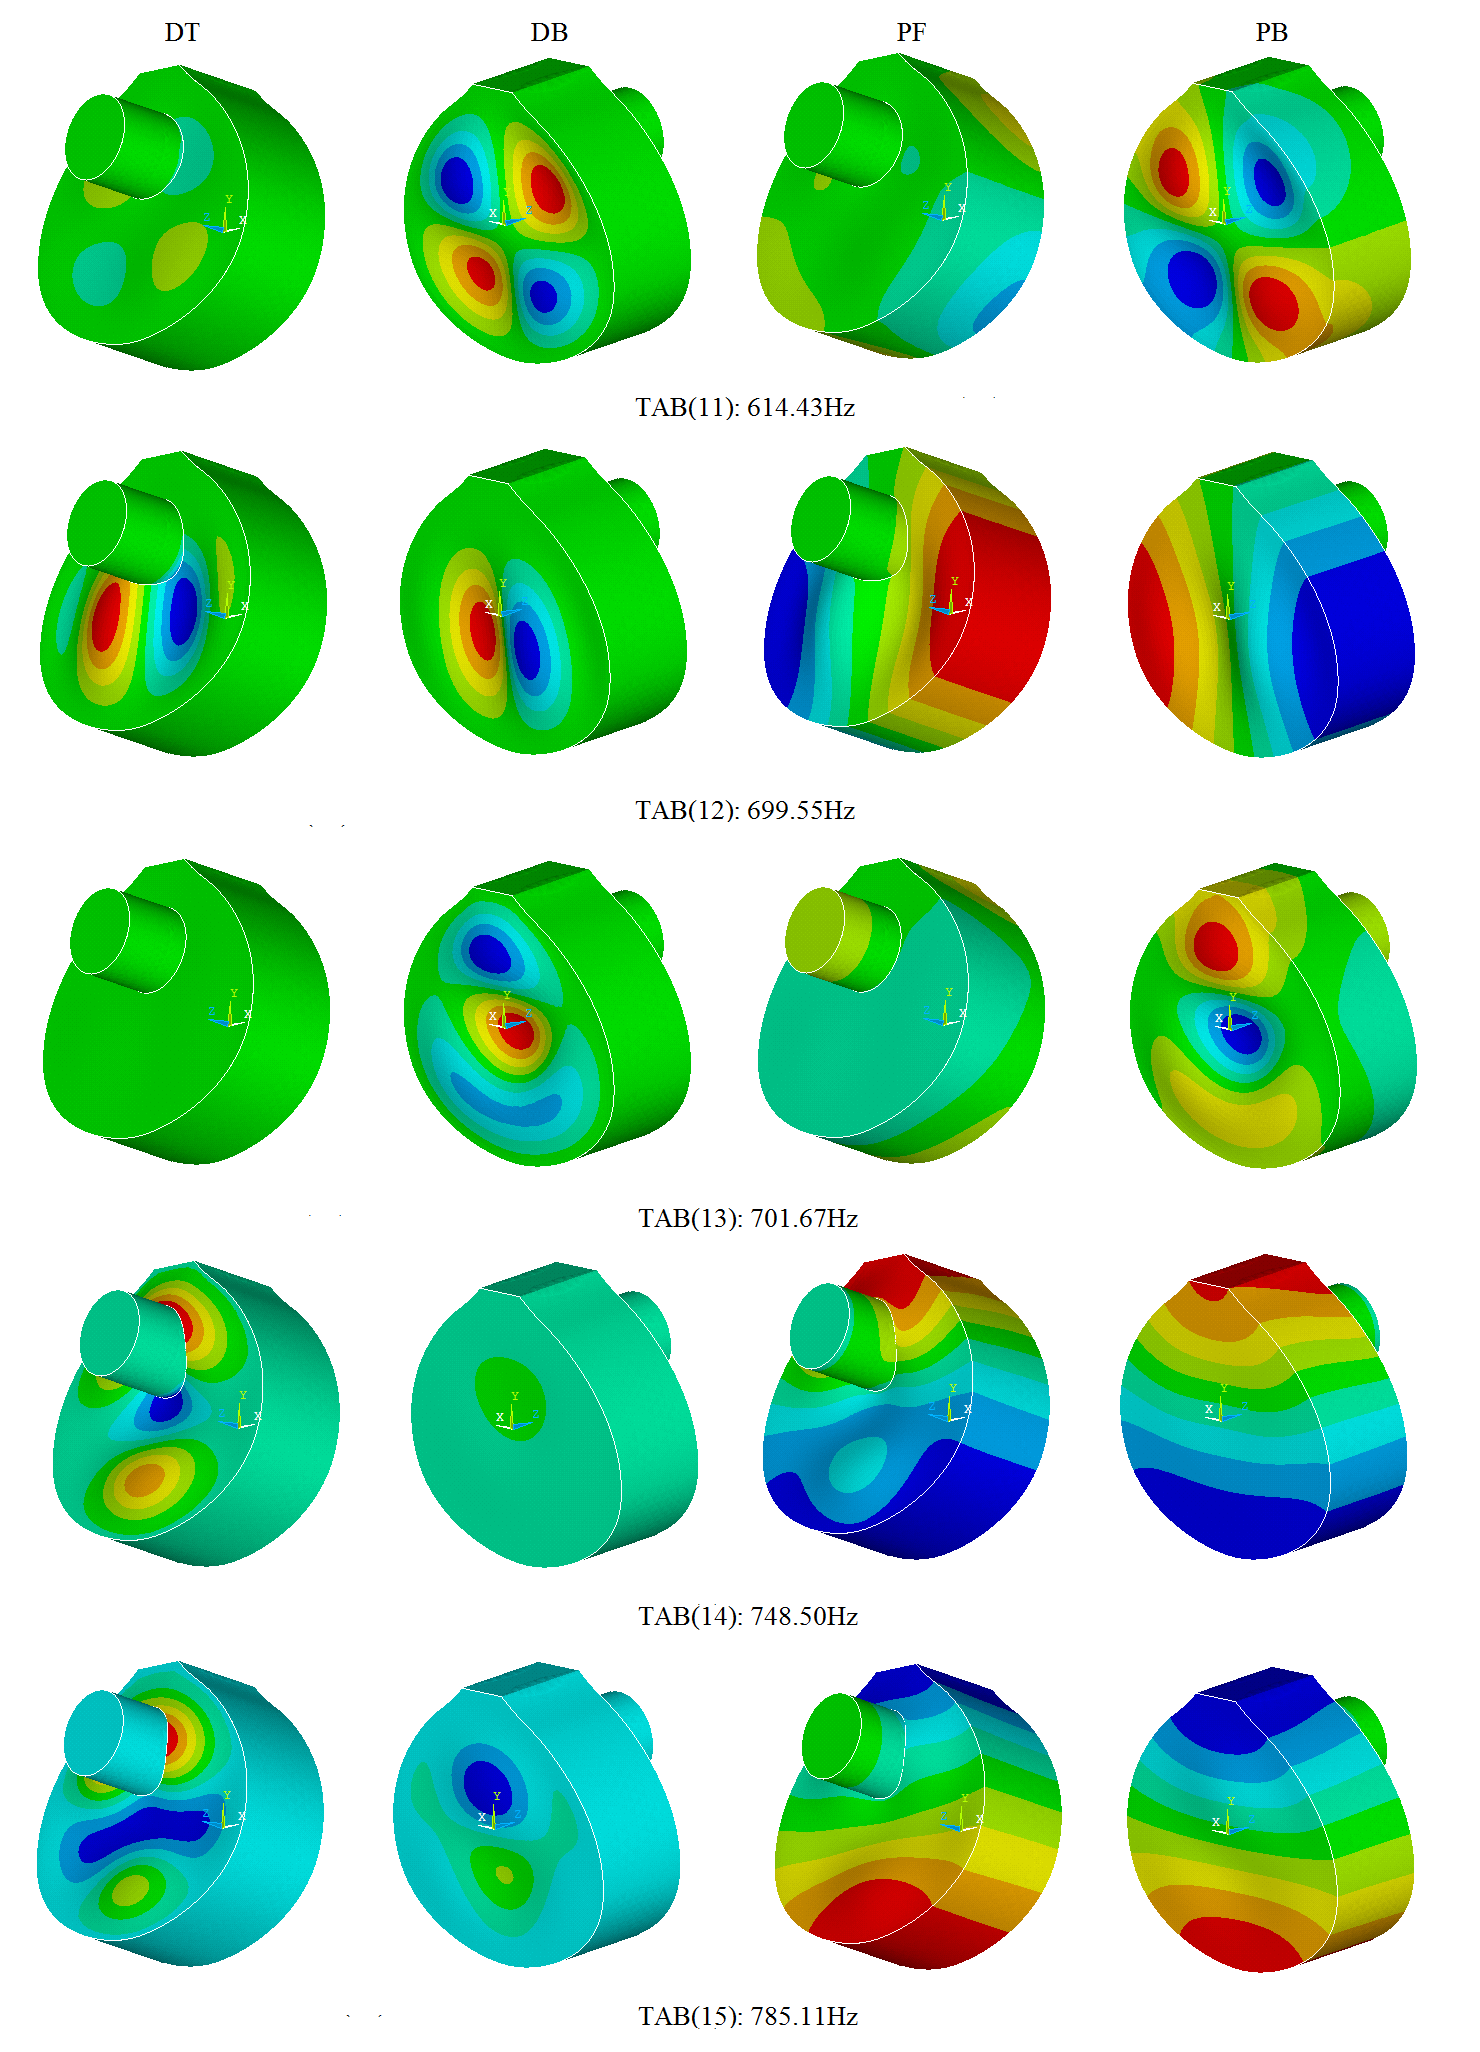
\includegraphics[height=9cm]{img/FSI3c.png}
\caption{Coupled modes of vibration for bandola's resonance box considering the oscillation of top plate, enclosed air and back plate}
\label{CoupledModes3c}
\end{figure}

It is observed in Figure \ref{CoupledModes3a} that TAB(1) presents clearly the same mode shapes of T(1,1) and B(1,1) in top and back plates respectively, and that A0 can be easily recognized in the pressure distribution. In this mode, top and back plate vibrate with opposite phases, moving outward and inward and changing considerably the volume of the resonance box. Due to this motion, the air is drawn and expelled from the cavity like a breathing. TAB(1) can be thus called, as in others instruments with resonance box, the "breathing mode" \cite{Pennstate}. Moreover, TAB(2) also presents the shapes of T(1,1) and B(1,1), however, the pressure distribution is very confusing and seems to be highly influenced by both shapes of top and back plate. This time the plates vibrate in phase and thus, the volume of resonance box will change a small amount that depends on the displacement amplitude of the plates, which in this case is greater for top plate. The third coupled mode TAB(3) doesn't have the same problem of identifying the mode that governs pressure distribution: A0 is easily recognized, although a greater pressure variation is present throughout the cavity. The mode shapes in top and back plate are also related to T(1,1) and B(1,1), but now the mode in the back plate present a bigger area of displacement. The motion between both plates is again in opposite phase.

According to the model of coupling with three oscillators, these three lowest modes TAB(1), TAB(2) and TAB(3) show the influence of mainly T(1,1), B(1,1) and A0. In each case, one of the uncoupled modes is dominant over the others, for instance, A0 drives the first coupled mode, T(1,1) drives the second and B(1,1) drives the third. Additionally, these modes seem to be efficient radiators although this is also determined by the phase of piston air. Thus, it would be convenient some experimental measurements in the bandola.

By examining TAB(1), TAB(2) and TAB(3), it can be observed that $f_1<f_h$, $f_2<f_p$ and $f_3>f_b$ where $f_b>f_p>f_h$. In comparison with the two lowest modes TA(1) and TA(2) predicted by the model of two oscillators, the frequencies of TAB(1) and TAB(2) decreased in value as if the effect of considering the back plate was that of an added mass. For guitars, Meyer and Elejabarrieta \cite{Elejabarrieta, Elejabarrieta1} have reported the same behavior when considering the vibration of back plate, however, Christensen \cite{Christensen3} has clarified that the second coupled resonance TAB(2) may be moved either upward (for $f_b<f_p$) or downward (for $f_b>f_p$), depending upon the uncoupled resonance frequencies $f_b$ and $f_p$ of the top and back plate.\\Verifying the expression in E.q.\ref{Combination3} it is found that:
\begin{eqnarray*}
\sqrt{f_p^2 + f_h^2 + f_b^2} & = & 322.66 \text{Hz}\\
\sqrt{f_1^2 + f_2^2 + f_3^2} & = & 351.65 \text{Hz}.
\end{eqnarray*}
These results are consistent since the percent error, relative to the sum of coupled terms, is 8.24\%. With this result, the next step would be an experimental validation, as suggested before.

By observing all coupled modes that were calculated, it is noted that the combination of the uncoupled modes of the plates and the air produces the coupled modes, all lying into the frequency range of 0-800Hz. However, only at the lowest five modes is achieved a strong coupling between the modes of the top plate, the enclosed air and the back plate. The rest of the modes could present a coupling between the top plate and the air alone or almost vibrate separately. This coupling could be thought to have a repulsive effect on the modes with increasing frequency.   

Dynamic response (into a specific frequency range) of a complex structure may be described by the combination of the modes of each substructure (all lying in the same frequency range) \cite{Ewins}, therefore, a model considering fifteen uncoupled oscillators, three representing the modes of air inside the cavity, six representing the modes of the top plate and other six for the modes of the back plate, could predict the fifteen calculated coupled modes. 
